\chapter{Transfer Function Optimization Using Visibility-Weighted Saliency}

\section{Introduction}
Volume visualization is an effective means of discovering meaningful features in volume data sets.
Both the exterior and interior of structures can be revealed simultaneously in a semi-transparent manner by specifying opacity values for the features in transfer functions.
Features can be intensity intervals in 1D transfer functions, rectangular or other shapes in 2D or higher-dimensional transfer functions.

In the specification of transfer functions for volume visualization, users often have a rough idea of how clear and opaque each feature should be and then adjust the opacity value of the features accordingly.
However, the relationship between the opacity of features and the saliency of the features in the final image is not linear.
The saliency of a feature in the final image depends on the opacity value assigned to the feature as well as the neighborhood of the feature and view-dependent occlusion of the feature.

Therefore, it is desirable to have an automated method to assist the user in the design of transfer functions. In this chapter, we propose an optimization approach to automatically refine a user-defined transfer function towards target saliency levels specified by the user.

%-------------------------------------------------------------------------
\section{Method}
In Chapter~\ref{visibility-weighted_saliency}, visibility-weighted saliency was proposed as a measure of visual saliency of features in volume rendered images, in order to assist users in choosing suitable viewpoints and designing effective transfer functions to visualize the features of interest. In this chapter, we describe a transfer function optimization approach based on the visibility-weighted saliency metric, which indicates the perceptual importance of voxels and the visibility of features in volume rendered images.

The approach described in Chapter~\ref{transfer_function_refinement} is an automated method of optimizing transfer functions, based on the intensity distribution of voxels in the volume data set. However, this approach does not take into account the spatial distribution of voxels and the viewpoint of the visualization. Visibility-weighted saliency, on the other hand, takes into account both of these two aspects. The visibility-weighted saliency consists of two component fields, i.e. saliency field and visiblity fields. Saliency fields are essentially difference of Gaussians, which include the information of local neighborhoods of voxels, and visibility fields are computed from opacity contribution of voxels to volume rendered images, which indicate viewpoint dependent occlusions of the voxels.

\subsection{Objective Function}
Users define target importance values for each feature defined in the transfer function domain.
Our approach adjusts the transfer function to match the visibility-weighted saliency with the user-defined target saliency values.
Multiple saliency fields computed from different appearance attributes can be combined together in order to represent different aspects of the visual saliency of voxels.
In our implementation, brightness and saturation are used respectively to compute visibility-weighted saliency fields and define the weighted sum of the two sets of feature saliency as visibility-weighted feature saliency.
The objective function is defined as the root mean square of the differences of the visibility-weighted saliency and target importance of each feature.
\[ f=\sqrt{ \frac{\sum_{i=1}^{n} (W_{i}-t_{i})^{2}}{n} } 
\addtag \]
where $ W_{F}=u_{1}W_{F}(O_{b},i,\sigma)+u_{2}W_{F}(O_{s},i,\sigma) $ is the visibility-weighted saliency of feature $ i $, as previously described in Section~\ref{weighted_feature_saliency}. $ t_{i} $ is the user-defined importance of feature $ i $. These user-defined saliency values are normalized and they add up to 1, in other words, $ t_{i} \in [0.1] $ and $ \sum_{i=1}^{n} t_{i} = 1 $.

\subsection{The Mapping from Opacity to Visibility-Weighted Saliency}
However, the visibility-weighted saliency $ W_{i} $ is not a variable that can be directly modified. Instead, $ W_{i} $ is a complicated function dependent on the opacity values of features, the spatial distribution of voxels and the viewpoint of the visualization.
We use a nucleon data set to demonstrate how the visibility-weighted saliency of features change when the feature opacity values change. As displayed in Figure~\ref{fig:nucleon_naive}, three features are defined in the transfer function for the nucleon data set.
In order to provide an intuitive overview of the relationship between the feature opacity values and the visibility-weighted saliency values, the 3 feature opacity values are mapped to $ x, y, z $ axes. Feature 1 (purple) in Figure~\ref{fig:nucleon_naive} is the exterior of the nucleon data set, the visibility-weighted saliency of this feature is shown in the 3D scalar fields in the same color at the left in Figure~\ref{fig:nucleon_densityplot}. The visibility-weighted saliency of feature 1 increases as the opacity increases, as shown in the figure that the brightness and opacity increase along $ x $ axis. Because feature 1 is the exterior, its visibility-weighted saliency is almost not affected by the opacity of other features. On the other hand, the visibility-weighted saliency of feature 2 (red) in Figure~\ref{fig:nucleon_naive} is affected by both the opacity of feature 1 and feature 2. In addition, the visibility-weighted saliency of feature 3 (green) in Figure~\ref{fig:nucleon_naive} is affected by the opacity of feature 1, feature 2 and feature 3.

In order to demonstrate the how the objective function change in the search space $ x \in [0,1] $, $ y \in [0,1] $ and $ z \in [0,1] $, we sample the search space with sampling interval $ 0.1 $, from 0 to 1 along each axis. That's 11 points along each axis, which results in 1331 sample points in the search space. In Figure~\ref{fig:nucleon_searchspace}, the search space is rendered as a density plot with a temperate color map which gradually changes from orange to blue.

\begin{figure}
\centering
	\begin{minipage}{.3\textwidth}
	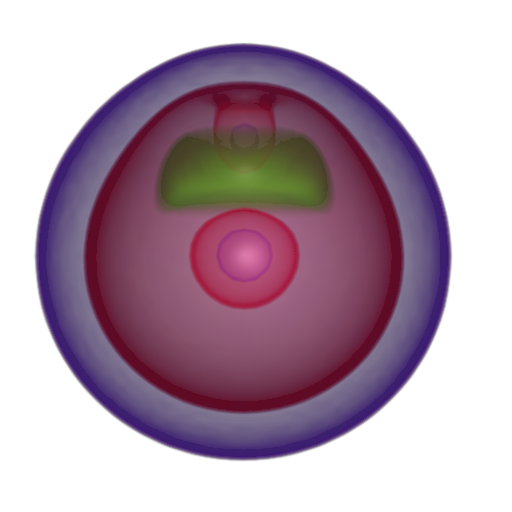
\includegraphics[width=1\linewidth]{images/nucleon_naive}
	\end{minipage}~
	\begin{minipage}{.3\textwidth}
	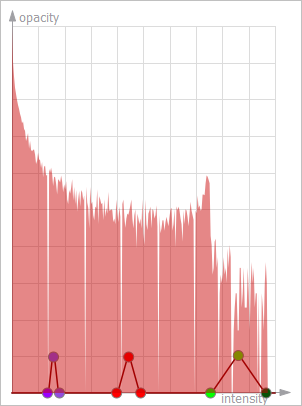
\includegraphics[width=1\linewidth]{images/tf_nucleon_naive}
	\end{minipage}
	\caption{A nucleon data set \cite{website:Voreen_datasets_2013} (left) with a transfer function of equal opacity values to the 3 features (right)}
	\label{fig:nucleon_naive}
\end{figure}

\begin{figure}
	\centering
	\begin{minipage}{.3\textwidth}
		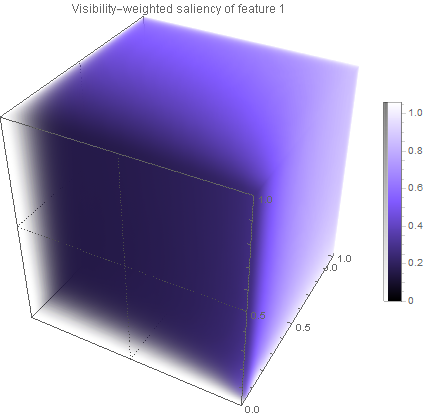
\includegraphics[width=1\linewidth]{images/densityplot1}	
	\end{minipage}~
	\begin{minipage}{.3\textwidth}
		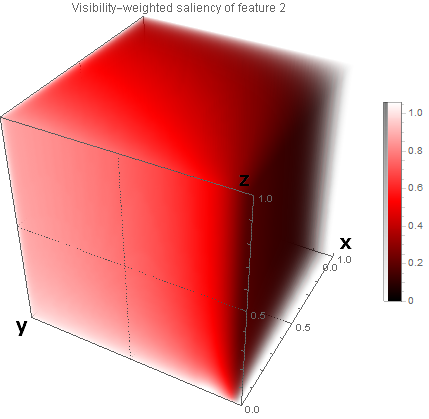
\includegraphics[width=1\linewidth]{images/densityplot2}	
	\end{minipage}
	\begin{minipage}{.3\textwidth}
		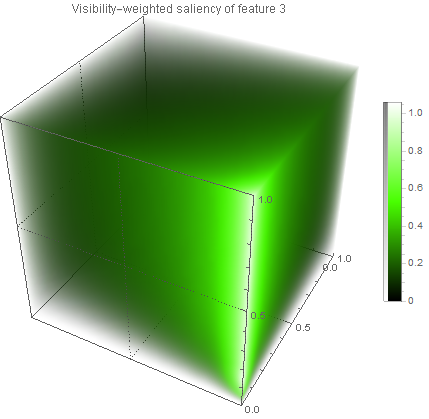
\includegraphics[width=1\linewidth]{images/densityplot3}	
	\end{minipage}
	\caption{Visibility-weighted saliency of the 3 features are mapped to brightness and opacity of the 3D fields at the left, middle and right respectively. The visibility-weighted saliency of feature 2 (red) is affected by both the opacity of feature 1 (purple) and feature 2. The visibility-weighted saliency of feature 3 (green) is affected by the opacity of feature 1, feature 2 and feature 3.}
	\label{fig:nucleon_densityplot}
\end{figure}

\begin{figure}
	\centering
	\begin{minipage}{.6\textwidth}
		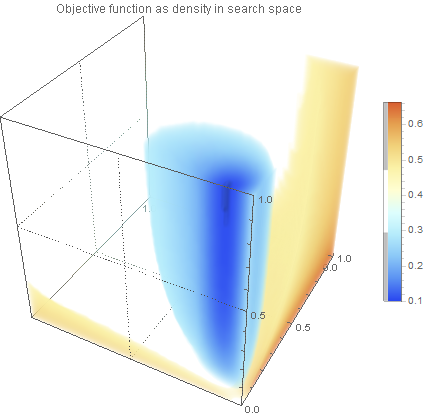
\includegraphics[width=1\linewidth]{images/searchspace}
	\end{minipage}
	\caption{The value of the objective function $  f $ is displayed as the density in the search space. Target saliency values are  0.1, 0.3 and 0.6 for the 3 features respectively.}
	\label{fig:nucleon_searchspace}
\end{figure}


\subsection{Optimization Algorithm}


\subsection{Adaptive Step Size with Line Search}
Line search is a procedure to adapt the step size in gradient descent in order to achieve a reduction in the objective fuction while still making sufficiently fast progress. Line search in employed in many multivariate optimization algorithms.
The input to a line search is an objective function $ f $, an initial point $ x $, direction $ d $ and an initial step size $ s $.

\subsection{Adaptive Step Size with Parallel Search}
Parallel computation has overhead.
It's worthy to perform line search in parallel when the evaluation of the objective function is computational expensive.
Computing the visibility fields is require to perform a pass of slice-based volume rendering, which is computational expensive.

%-------------------------------------------------------------------------
\section{Results and Discussions}

\begin{figure}
	\centering
	\begin{minipage}{.9\textwidth}
		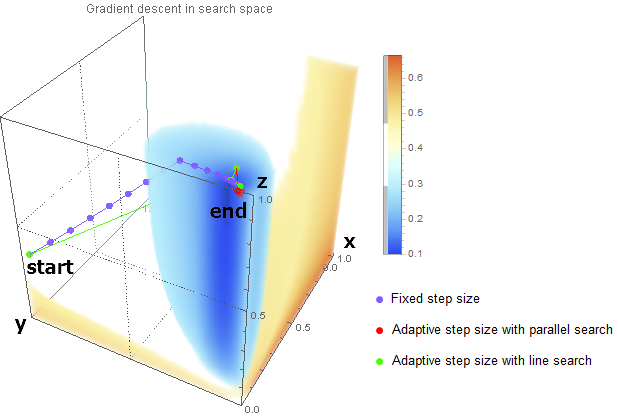
\includegraphics[width=1\linewidth]{images/searchspace_path}
	\end{minipage}
	\caption{Search space}
	\label{fig:nucleon_searchspace_path}
\end{figure}

\begin{figure}
	\centering
	\begin{minipage}{.3\textwidth}
		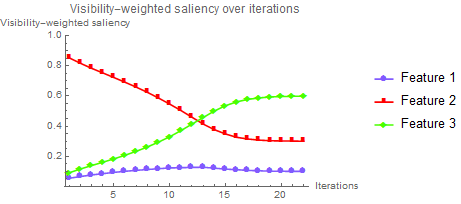
\includegraphics[width=1\linewidth]{images/saliency_fixed}
		\caption{a}	
	\end{minipage}~
	\begin{minipage}{.3\textwidth}
		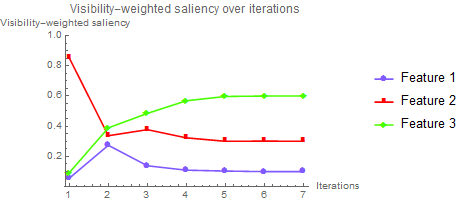
\includegraphics[width=1\linewidth]{images/saliency_linesearch}
		\caption{b}	
	\end{minipage}
	\begin{minipage}{.3\textwidth}
		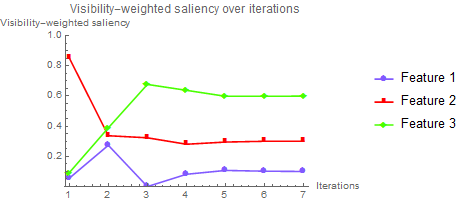
\includegraphics[width=1\linewidth]{images/saliency_parallelsearch}
		\caption{b}	
	\end{minipage}
	\label{fig:nucleon_saliency}
\end{figure}

\begin{figure}
	\centering
	\begin{minipage}{.3\textwidth}
		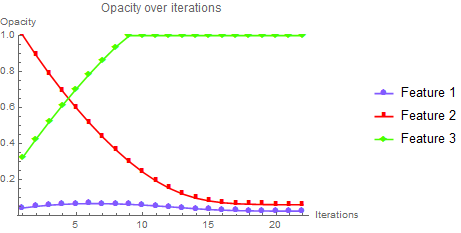
\includegraphics[width=1\linewidth]{images/opacity_fixed}
		\caption{a}	
	\end{minipage}~
	\begin{minipage}{.3\textwidth}
		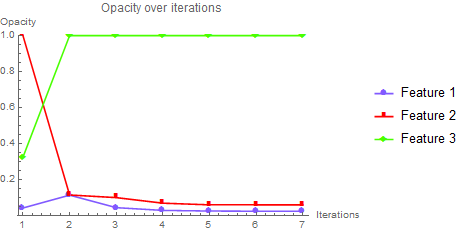
\includegraphics[width=1\linewidth]{images/opacity_linesearch}
		\caption{b}	
	\end{minipage}
	\begin{minipage}{.3\textwidth}
		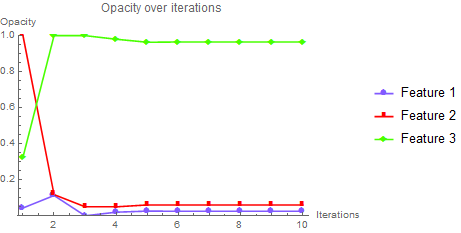
\includegraphics[width=1\linewidth]{images/opacity_parallelsearch}
		\caption{b}	
	\end{minipage}
	\label{fig:nucleon_opacity}
\end{figure}

\begin{figure}
	\centering
	\begin{minipage}{.3\textwidth}
		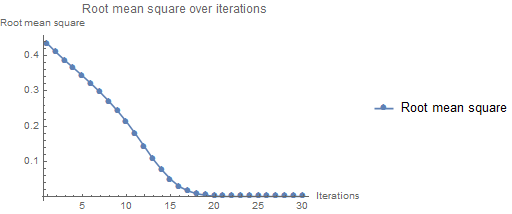
\includegraphics[width=1\linewidth]{images/rms_fixed}
		\caption{a}	
	\end{minipage}~
	\begin{minipage}{.3\textwidth}
		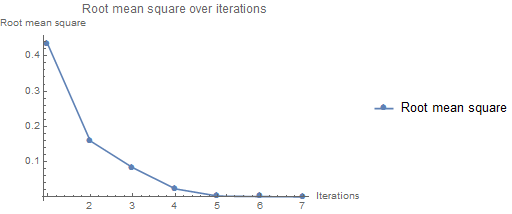
\includegraphics[width=1\linewidth]{images/rms_linesearch}
		\caption{b}	
	\end{minipage}
	\begin{minipage}{.3\textwidth}
		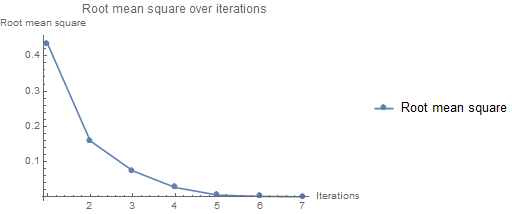
\includegraphics[width=1\linewidth]{images/rms_parallelsearch}
		\caption{b}	
	\end{minipage}
	\label{fig:nucleon_rms}
\end{figure}

%-------------------------------------------------------------------------
\section{Conclusions}
